\documentclass[10pt]{article}
% Эта строка — комментарий, она не будет показана в выходном файле
\usepackage{ucs}
\usepackage[utf8x]{inputenc} % Включаем поддержку UTF8
\usepackage[russian]{babel}  % Включаем пакет для поддержки русского языка
\usepackage{amsmath}
\usepackage{amssymb}
\usepackage{mathtools}

\hoffset=0mm
\voffset=0mm
\textwidth=170mm        % ширина текста
\oddsidemargin=-0mm   % левое поле 25.4 - 5.4 = 20 мм
\textheight=240mm       % высота текста 297 (A4) - 40
\topmargin=-15.4mm      % верхнее поле (10мм)
\headheight=5mm      % место для колонтитула
\headsep=5mm          % отступ после колонтитула
\footskip=8mm         % отступ до нижнего колонтитула



% \textwidth=180mm    
% \oddsidemargin=-10mm 

\title{Лабораторная работа № 2.2: {\it Изучение вынужденных колебаний в колебательном контуре.}}
\author{Зотов Алексей, 497}
\date{\today}

\begin{document}

\maketitle
\textbf{Цель работы:} изучение зависимости тока в колебательном контуре от частоты источника ЭДС, включенного в контур, и измерение резонансной частоты контура.

\textbf{В работе испольуются:} \small{звуковой генератор Г6–46, электронныйосциллограф, модуль ФПЭ–11, магазин сопротивлений, магазин емкостей.}

\textbf{Ход работы:}
    \begin{enumerate}
    \item \textbf{Снятие резонансных кривых.} \\
        $C = 3$нФ, $R_1 = 75$Ом. \\
        Найдем зависимость $U_0$ и $I_0$ от частоты $f$. 
        \small{
        \begin{enumerate}
            \item $R = 1$ Ом \\
            $f = [2,3,4,5,6,6.5,6.7,6.9,7.0,7.1,7.3,7.5,7.7,8,10,12,14,16]$ кГц \\
            $U_0 = [8,12,16,28,56,90,120,155,167,170,160,145,128,100,40,25,19,15]$ мВ \\
            $I_0 = \frac{U_0}{R_1} = [ 0.11,  0.16,  0.21,  0.37,  0.75,  1.2 ,  1.6 ,  2.07,  2.23,
         2.27,  2.13,  1.93,  1.71,  1.33,  0.53,  0.33,  0.25,  0.2 ]$ мА \\

            \item $R = 1$ Ом \\
            $f = [2,4,6,6.5,6.7,6.8,6.9,7.0,7.1,7.2,7.4,7.6,7.8,8,9,10,12,14,16]$ кГц \\
            $U_0 = [8,16,52,75,90,100,108,112,120,120,119,110,100,90,57,40,24,18,15]$ мВ \\
            $I_0 = \frac{U_0}{R_1} = [ 0.11,  0.21,  0.69,  1.  ,  1.2 ,  1.33,  1.44,  1.49,  1.6 ,
         1.6 ,  1.59,  1.47,  1.33,  1.2 ,  0.76,  0.53,  0.32,  0.24,  0.2 ]$ мА \\

         \item $R = 1$ Ом \\
            $f = [2,4,6,6.5,6.7,6.9,7.1,7.3,7.5,7.7,8,10,12,14,16]$ кГц \\
            $U_0 = [8,17,36,40,43,44,45,47,47,46,44,30,23,18,14]$ мВ \\
            $I_0 = \frac{U_0}{R_1} = [ 0.11,  0.23,  0.48,  0.53,  0.57,  0.59,  0.6 ,  0.63,  0.63,
         0.61,  0.59,  0.4 ,  0.31,  0.24,  0.19]$ мА \\
        \end{enumerate}
        }

        \begin{center}
        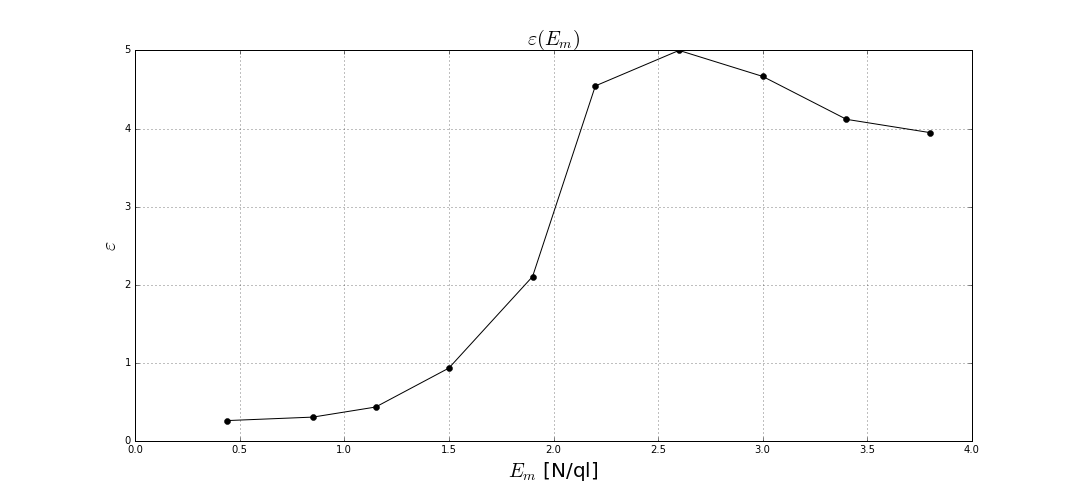
\includegraphics[width=14cm,height=6cm]{plot2.png}
        \end{center}

        Резонансная частота $f_r \approx 7.1$ кГц. \\
        Используя приблизительное значение индуктивности $L = 100$ мГн, рассчитаем резонансную частоту контура теоретчиески:
        \begin{equation}
            f^{th}_{r} = \frac{1}{2 \pi \sqrt{LC}} \approx 9.2 \text{кГц}
        \end{equation} 
        что по порядку совпадает с частотой, полученной в эксперименте. \\
        Найдем ширину резонансной кривой $\Delta f$ и рассчитаем значения добротности: 
        \begin{enumerate}
        \item $R = 1$ Ом \\
            $\Delta f \approx 1.2$ кГц , $Q = \frac{f_r}{\Delta f} \approx 6.2$
        \item $R = 500$ Ом \\
            $\Delta f \approx 1.5$ кГц , $Q = \frac{f_r}{\Delta f} \approx 4.7$
        \end{enumerate}
        Как и ожидалось, система с большим сопротивлением имеет меньшую добротность.
        
    \item \textbf{Определение зависимости резонансной частоты от емкости.} \\
        $R = 1$ Ом \\
        Найдем зависимость резонансной частоты $f_r$ от емкости $C$: \\
        $C = [1,  2,  3 , 4 , 5 , 6 , 7 , 8 , 9 ,10]$ нФ \\
        $f_r = [12.1, 8.78, 7.12, 6.09, 5.5, 5.06, 4.66, 4.39, 4.12, 3.92]$ кГц \\
        \begin{equation} 
            F := \frac{1}{(2 \pi f_r)^2}
        \end{equation}
        $F = [ 0.17 , 0.33 , 0.50 , 0.68 , 0.84 , 0.99 1.17 , 1.31 , 1.49 , 1.65] \cdot 10 ^{-9}$ [$\text{c}^2$] 
        \begin{center}
        \includegraphics[width=14cm,height=6cm]{plot3.png}
        \end{center}

        Найдем индуктивность катушки $L$ :
        \begin{equation}
            F = \frac{1}{(2 \pi f_r)^2} = LC \implies L = \frac{dF}{dC} = \frac{F}{C}.
        \end{equation}
        \begin{equation}
            L = \frac{1}{n} \sum^{n}_{i=1} \frac{F_i}{C_i} = 0.167 \pm 0.003 \quad \text{Гн}
        \end{equation}
        Рассчет погрешности: \\
        $\sigma_f = 0.02$ кГц $\implies \varepsilon_f \approx 0.4 \% $ \\
        $ \varepsilon_F = 2 \varepsilon_f $ \\
        $\varepsilon_C = 5 \% $ \\
        \begin{equation}
        \varepsilon_{\frac{F_i}{C_i}} = \sqrt{\varepsilon^2_{C_i} + \varepsilon^2_{F_i}}
        \end{equation}
        \begin{equation}
        \sigma_{\frac{F_i}{C_i}} = \frac{F_i}{C_i} \cdot \varepsilon_{\frac{F_i}{C_i}}
        \end{equation}
        \begin{equation}
        \sigma_{L} = \frac{1}{n} \sqrt{\sum^n_{i=1} \sigma_{\frac{F_i}{C_i}} ^ 2} \approx 0.003 \text{ Гн}\
        \quad \varepsilon_{L} \approx 1.6 \%
        \end{equation}

    \end{enumerate}

\end{document}

